\section{Experimentos e resultados}
\subsection{Experimentos}
A fim de poder entender o funcionamento do simulador NS-2 e tamb\'em estudar simula\c{c}\~oes de comunica\c{c}\~ao em cen\'arios militares, foram definidos 2 experimentos te\'oricos, sendo o Experimento 1, um teste simples de converg\^encia de rotas, e o Experimento 2, baseado em estudos realizados por \cite{pereira}, o qual representa um caso de assalto e tomada de posi\c{c}\~ao inimiga.

Cada experimento possui suas caracter\'isticas, mas exitem uma semalhan\c{c}a base, que \'e o tr\'afego que ir\'a caminhar pela rede, como ja comentado na se\c{c}\~ao \ref{trafegoDados}, o qual foi escolhido o CBR.

\subsubsection{Experimento 1}
O experimento 1 baseia-se na ideia simples de um protocolo de rede \textit{ad hoc}, roteamento din\^amico.
O objetivo principal deste experimento \'e poder analizar o tempo de converg\^encia de roteamento de uma origem a um destino, alterando uma vez o caminho pelo qual eles realizam a comunica\c{c}\~ao.

\begin{table}[H]
	\centering
	\caption{Resumo dos par\^ametros usados no Experimento 1.}
	\begin{tabular}{ | l | l | }
		\hline
		N\'umero total de n\'os & 4 \\ \hline
		N\'umero de fontes de tr\'afego & 1 \\ \hline
		Tempo de simula\c{c}\~ao & 300 segundos \\ \hline
		\'Area total da simula\c{c}\~ao & 500x500 metros \\ \hline
		Velocidade dos n\'os & 1.5m/s constante \\ \hline
		Valocidade de banda & 11Mbps/s \\ \hline
	\end{tabular}
	\label{tabParamExp1}
\end{table}

A Figura \ref{figExp1} demonstra o experimento realizado, onde cada Soldado(n\'o) deve atingir seu respectivo Destino.
Cada Soldado inicia seu movimento a um tempo determinado na simula\c{c}\~ao, onde na Figura \ref{figExp1} \'e referenciado pelo prefixo \textit{at}, o qual \'e defido em segundos, e abaixo exibe o movimento de cada Soldado, onde nesse experimento todos os Soldados possuem um movimento constante de 1,5 metros por segundo. 

A fonte de tr\'afego nesse experimento \'e somente de uma, a qual realiza uma conex\~ao do Soldado 3(fonte) ao Soldado 1(destino). Inicialmente vai passar pelo Soldado 2 essa comunica\c{c}\~ao, pois os Soldados 1 e 3 n\~ao est\~ao pr\'oximos a fim de criarem uma rota direta.

\begin{figure}[H]
	\centering
	\includegraphics[scale=0.5]{experimento1.eps}
	\caption{Experimento 1}
	\label{figExp1}
\end{figure}

Observe que o Soldado 4 inicia somente seu movimento ao tempo de 150,0 segundos, enquanto os demais Soldados iniciam seus movimentos ao instante de 0,1 segundos.
Isso foi definido pelo fato do tempo em que o Soldado 2 atinja seu objetivo e pare de seguir em frente, enquanto os Soldados 1 e 3 continuam seus movimentos, e possam alcan\c{c}ar e estar dentro do raio de comunica\c{c}\~ao com o Soldado 4.
Quando os Soldados 1 e 3 se afastam do Soldado 2, eles perdem a sua rota por esse \textit{host} da rede, e necessitam buscar uma nova rota, a qual seguir\'a pelo Soldado 4, e \'e nesse ponto onde cada protocolo dever\'a gerar resultados distintos.

\subsubsection{Experimento 2}
Isso \'e o exemplo do experimento 2.

Ele consiste em analizar o fuxo da rede passante.

\begin{figure}[H]
	\centering
	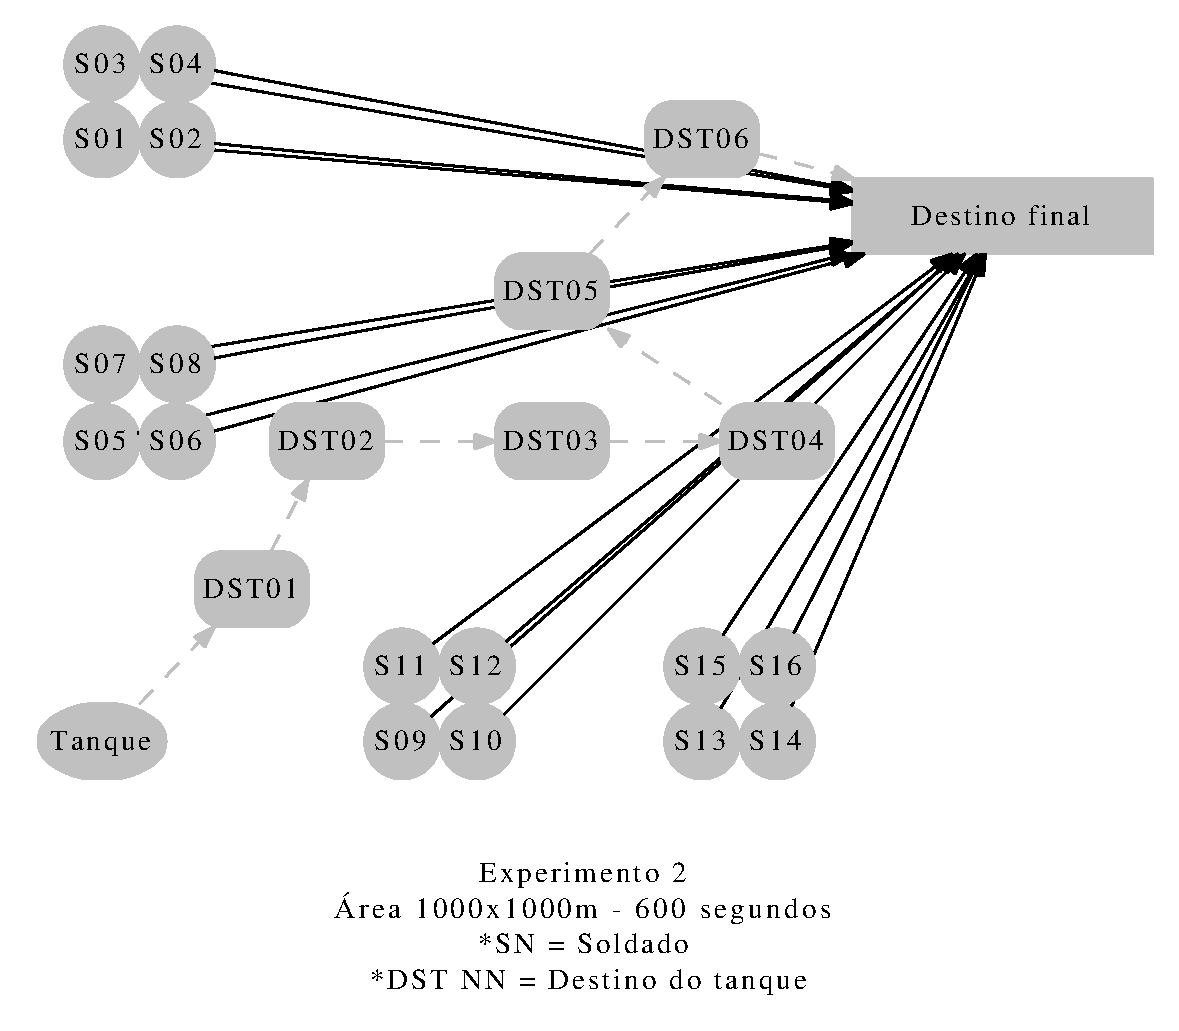
\includegraphics[scale=0.5]{experimento2.eps}
	\caption{Experimento 2}
	\label{figExp2}
\end{figure}


\subsection{M\'etricas de desempenho}
Com base nos estudo de \cite{pereira} e \cite{schimidt} e informa\c{c}\~oes obtidas por \cite{salles}, foram definidas m\'etricas para analizar o comportamento de cada protocolo e poder tamb\'em comparar resultados obtidos em estudos anteriores j\'a realizados pelos 2 primeiros autores citados.

\begin{itemize}
	\item \textbf{Taxa de entrega de pacotes:} Raz\~ao entre o n\'umero de pacotes entregues para o destino final e o n\'umero de pacotes gerados pela aplica\c{c}\~ao na fonte.
	\item \textbf{Atraso m\'edio fim a fim dos pacotes de dados:} Inclui todos os poss\'iveis atrasos causados pela lat\^encia da descoberta de rotas, propaga\c{c}\~ao, atrasos devido a retransmiss\~oes da camada MAC e tempos de transfer\^encia.
	\item \textbf{N\'umero de pacotes de roteamento:} \'E medido a quantidade total de pacotes de roteamento, representada pelos pacotes de descoberta e manuten\c{c}\~ao das rotas enviados pela origem ou encaminhados pelos n\'os intermedi\'arios. No protocolo por demanda (AODV), esses pacotes s\~ao representados pelos pacotes RREQ, RREP e RERR. No DSDV e OLSR, esses pacotes s\~ao representados pelas tabelas de roteamento que s\~ao trocadas periodicamente.
	\item \textbf{N\'umero de \textit{bytes} de roteamento:} \'E medido a quantidade total de \textit{bytes} em cada pacote de, incluindo a quantidade de \textit{bytes} de cabe\c{c}alho em pacotes de dados, que corresponde, normalmente, ao roteamento na fonte.
\end{itemize}
Segundo \cite{pereira}, o tr\'afego referente ao roteamento deve ser o menor poss\'ivel quando comparado ao tr\'afego de dados, pois para se enviar pacotes de roteamento gasta-se energia dos n\'os e consome-se banda, que s\~ao recursos escassos em redes sem fio. 
Para as redes militares, a taxa de entrega e o atraso s\~ao as m\'etricas mais importantes.

\subsection{An\'alise comparativa dos resultados}

\subsubsection{Experimento 1}

\begin{figure}[H]
	\centering
	\subfigure[Taxa de entrega de pacotes]{
		\includegraphics[scale=0.55]{lost.eps}
	}\label{subfig:exp1Lost}
	\subfigure[Atraso m\'edio (s)]{
		\includegraphics[scale=0.55]{delay.eps}
	}\label{subfig:exp1Late}
	\subfigure[N\'umero de \textit{bytes} de roteamento]{
		\includegraphics[scale=0.55]{byte.eps}
	}\label{subfig:exp1Byte}
	\subfigure[N\'umero de pacotes de roteamento]{
		\includegraphics[scale=0.55]{pkts.eps}
	}\label{subfig:exp1Pkts}
	
	\caption{Resultados para o experimento 1}
	\label{fig:resulExp1}
\end{figure}

\begin{table}[H]
	\centering
	\caption{Resultado das simula\c{c}\~oes do experimento 1}
	\begin{tabular}{ | l | l | l | l | }
		\hline
		M\'ETRICAS AVALIADAS & DSDV & AODV & OLSR \\ \hline
		Taxa de entrega & 92.98\% & 99.83\% & 98.43\% \\ \hline
		Atraso m\'edio (s) & 10.7575 & 11.4837 & 11.3047 \\ \hline
		N\'umero de pacotes & 543 & 588 & 565 \\ \hline
		N\'umero de \textit{bytes} & 288896 & 312816 & 300580 \\ \hline
	\end{tabular}
	\label{tabExp1Result}
\end{table}

\subsubsection{Experimento 2}

\begin{table}[H]
	\centering
	\caption{Resultado das simula\c{c}\~oes do experimento 2}
	\begin{tabular}{ | l | l | l | l | }
		\hline
		M\'ETRICAS AVALIADAS & DSDV & AODV & OLSR \\ \hline
		Taxa de entrega & XXX & XXX & XXX  \\ \hline
		Atraso m\'edio & XXX & XXX & XXX  \\ \hline
		N\'umero de pacotes & XXX & XXX & XXX  \\ \hline
		N\'umero de \textit{bytes} & XXX & XXX & XXX  \\ \hline
	\end{tabular}
	\label{tabExp2Result}
\end{table}
